\documentclass{article}\usepackage[]{graphicx}\usepackage[]{color}
%% maxwidth is the original width if it is less than linewidth
%% otherwise use linewidth (to make sure the graphics do not exceed the margin)
\makeatletter
\def\maxwidth{ %
  \ifdim\Gin@nat@width>\linewidth
    \linewidth
  \else
    \Gin@nat@width
  \fi
}
\makeatother

\definecolor{fgcolor}{rgb}{0.345, 0.345, 0.345}
\newcommand{\hlnum}[1]{\textcolor[rgb]{0.686,0.059,0.569}{#1}}%
\newcommand{\hlstr}[1]{\textcolor[rgb]{0.192,0.494,0.8}{#1}}%
\newcommand{\hlcom}[1]{\textcolor[rgb]{0.678,0.584,0.686}{\textit{#1}}}%
\newcommand{\hlopt}[1]{\textcolor[rgb]{0,0,0}{#1}}%
\newcommand{\hlstd}[1]{\textcolor[rgb]{0.345,0.345,0.345}{#1}}%
\newcommand{\hlkwa}[1]{\textcolor[rgb]{0.161,0.373,0.58}{\textbf{#1}}}%
\newcommand{\hlkwb}[1]{\textcolor[rgb]{0.69,0.353,0.396}{#1}}%
\newcommand{\hlkwc}[1]{\textcolor[rgb]{0.333,0.667,0.333}{#1}}%
\newcommand{\hlkwd}[1]{\textcolor[rgb]{0.737,0.353,0.396}{\textbf{#1}}}%

\usepackage{framed}
\makeatletter
\newenvironment{kframe}{%
 \def\at@end@of@kframe{}%
 \ifinner\ifhmode%
  \def\at@end@of@kframe{\end{minipage}}%
  \begin{minipage}{\columnwidth}%
 \fi\fi%
 \def\FrameCommand##1{\hskip\@totalleftmargin \hskip-\fboxsep
 \colorbox{shadecolor}{##1}\hskip-\fboxsep
     % There is no \\@totalrightmargin, so:
     \hskip-\linewidth \hskip-\@totalleftmargin \hskip\columnwidth}%
 \MakeFramed {\advance\hsize-\width
   \@totalleftmargin\z@ \linewidth\hsize
   \@setminipage}}%
 {\par\unskip\endMakeFramed%
 \at@end@of@kframe}
\makeatother

\definecolor{shadecolor}{rgb}{.97, .97, .97}
\definecolor{messagecolor}{rgb}{0, 0, 0}
\definecolor{warningcolor}{rgb}{1, 0, 1}
\definecolor{errorcolor}{rgb}{1, 0, 0}
\newenvironment{knitrout}{}{} % an empty environment to be redefined in TeX

\usepackage{alltt}
\usepackage{longtable} % needed for reporttools tables.
\usepackage{pdflscape} % for landscape pages.
\usepackage{hyperref}  % package used for hyperlinked toc.
\usepackage [toc, page]{appendix} % used for appendices
\usepackage{verbatim}
\IfFileExists{upquote.sty}{\usepackage{upquote}}{}


\begin{document}

\author{William Murrah}
\title{STAR Example Intent-to-treat Report}
\maketitle
\tableofcontents







\clearpage
\section{Introduction}

This is an example report of the \emph{STAR} data. The data consists of 100 cases and 10 variables. This example is a simplified version of the types of internal lab reports that can be generated using R and the \texttt{knitr} package to produce reproducible analyses. 

\clearpage
\begin{landscape}
\section{Descriptive Statistics}
% latex table generated in R 3.0.2 by xtable 1.7-1 package
% Sun Feb 16 14:42:51 2014
{\footnotesize
\begin{longtable}{ll|rrr|rrr|rrr}
 \textbf{Variable} & \textbf{Levels} & $\mathbf{n_{\mathrm{control}}}$ & $\mathbf{\%_{\mathrm{control}}}$ & $\mathbf{\sum \%_{\mathrm{control}}}$ & $\mathbf{n_{\mathrm{treatment}}}$ & $\mathbf{\%_{\mathrm{treatment}}}$ & $\mathbf{\sum \%_{\mathrm{treatment}}}$ & $\mathbf{n_{\mathrm{all}}}$ & $\mathbf{\%_{\mathrm{all}}}$ & $\mathbf{\sum \%_{\mathrm{all}}}$ \\ 
  \hline
gender & female & 20 & 39.2 & 39.2 & 28 & 57.1 & 57.1 & 48 & 48.0 & 48.0 \\ 
   & male & 31 & 60.8 & 100.0 & 21 & 42.9 & 100.0 & 52 & 52.0 & 100.0 \\ 
   \hline
$p= 0.11$ & all & 51 & 100.0 &  & 49 & 100.0 &  & 100 & 100.0 &  \\ 
   \hline
\hline
ethnicity & afam & 18 & 36.0 & 36.0 & 16 & 33.3 & 33.3 & 34 & 34.7 & 34.7 \\ 
   & cauc & 31 & 62.0 & 98.0 & 32 & 66.7 & 100.0 & 63 & 64.3 & 99.0 \\ 
   & hispanic & 1 & 2.0 & 100.0 & 0 & 0.0 & 100.0 & 1 & 1.0 & 100.0 \\ 
   \hline
$p= 0.58$ & all & 50 & 100.0 &  & 48 & 100.0 &  & 98 & 100.0 &  \\ 
   \hline
\hline
school1 & inner-city & 7 & 23.3 & 23.3 & 7 & 25.0 & 25.0 & 14 & 24.1 & 24.1 \\ 
   & rural & 14 & 46.7 & 70.0 & 12 & 42.9 & 67.9 & 26 & 44.8 & 69.0 \\ 
   & suburban & 6 & 20.0 & 90.0 & 7 & 25.0 & 92.9 & 13 & 22.4 & 91.4 \\ 
   & urban & 3 & 10.0 & 100.0 & 2 & 7.1 & 100.0 & 5 & 8.6 & 100.0 \\ 
   \hline
$p= 0.95$ & all & 30 & 100.0 &  & 28 & 100.0 &  & 58 & 100.0 &  \\ 
   \hline
\hline
degreek & bachelor & 17 & 63.0 & 63.0 & 16 & 64.0 & 64.0 & 33 & 63.5 & 63.5 \\ 
   & master & 8 & 29.6 & 92.6 & 7 & 28.0 & 92.0 & 15 & 28.9 & 92.3 \\ 
   & master+ & 2 & 7.4 & 100.0 & 2 & 8.0 & 100.0 & 4 & 7.7 & 100.0 \\ 
   \hline
$p= 0.99$ & all & 27 & 100.0 &  & 25 & 100.0 &  & 52 & 100.0 &  \\ 
   \hline
\hline
\hline
\caption{Descriptive Statistics for Qualitative Variables} 
\label{}
\end{longtable}
}


\clearpage
% latex table generated in R 3.0.2 by xtable 1.7-1 package
% Sun Feb 16 14:42:51 2014
{\footnotesize
\begin{longtable}{llrrrrrrrrrr}
 \textbf{Variable} & \textbf{Levels} & $\mathbf{n}$ & \textbf{Min} & $\mathbf{q_1}$ & $\mathbf{\widetilde{x}}$ & $\mathbf{\bar{x}}$ & $\mathbf{q_3}$ & \textbf{Max} & $\mathbf{s}$ & \textbf{IQR} & \textbf{\#NA} \\ 
  \hline
readk & control & 26 & 405.0 & 422.5 & 438.0 & 437.8 & 449.2 & 483.0 & 20.3 & 26.8 & 25 \\ 
   & treatment & 22 & 405.0 & 428.0 & 433.5 & 444.0 & 455.8 & 518.0 & 29.2 & 27.8 & 27 \\ 
   \hline
$p= 0.40$ & all & 48 & 405.0 & 427.0 & 436.5 & 440.6 & 450.2 & 518.0 & 24.7 & 23.2 & 52 \\ 
   \hline
read1 & control & 27 & 425.0 & 477.5 & 521.0 & 520.0 & 558.5 & 604.0 & 50.3 & 81.0 & 24 \\ 
   & treatment & 26 & 430.0 & 501.5 & 540.0 & 536.1 & 577.0 & 651.0 & 53.8 & 75.5 & 23 \\ 
   \hline
$p= 0.27$ & all & 53 & 425.0 & 483.0 & 536.0 & 527.9 & 571.0 & 651.0 & 52.2 & 88.0 & 47 \\ 
   \hline
mathk & control & 26 & 375.0 & 445.2 & 473.0 & 473.2 & 494.0 & 559.0 & 39.5 & 48.8 & 25 \\ 
   & treatment & 22 & 384.0 & 468.0 & 475.5 & 489.5 & 516.5 & 602.0 & 49.3 & 48.5 & 27 \\ 
   \hline
$p= 0.21$ & all & 48 & 375.0 & 452.8 & 473.0 & 480.7 & 506.0 & 602.0 & 44.6 & 53.2 & 52 \\ 
   \hline
math1 & control & 30 & 468.0 & 512.0 & 523.0 & 526.8 & 537.2 & 601.0 & 31.9 & 25.2 & 21 \\ 
   & treatment & 26 & 467.4 & 524.6 & 551.0 & 555.9 & 588.8 & 667.0 & 50.3 & 64.2 & 23 \\ 
   \hline
$p= 0.01$ & all & 56 & 467.4 & 515.0 & 533.5 & 540.3 & 568.7 & 667.0 & 43.6 & 53.8 & 44 \\ 
   \hline
\hline
\caption{Descriptive Statistics for Qauntitative Variables} 
\label{}
\end{longtable}
}


\end{landscape}
\clearpage

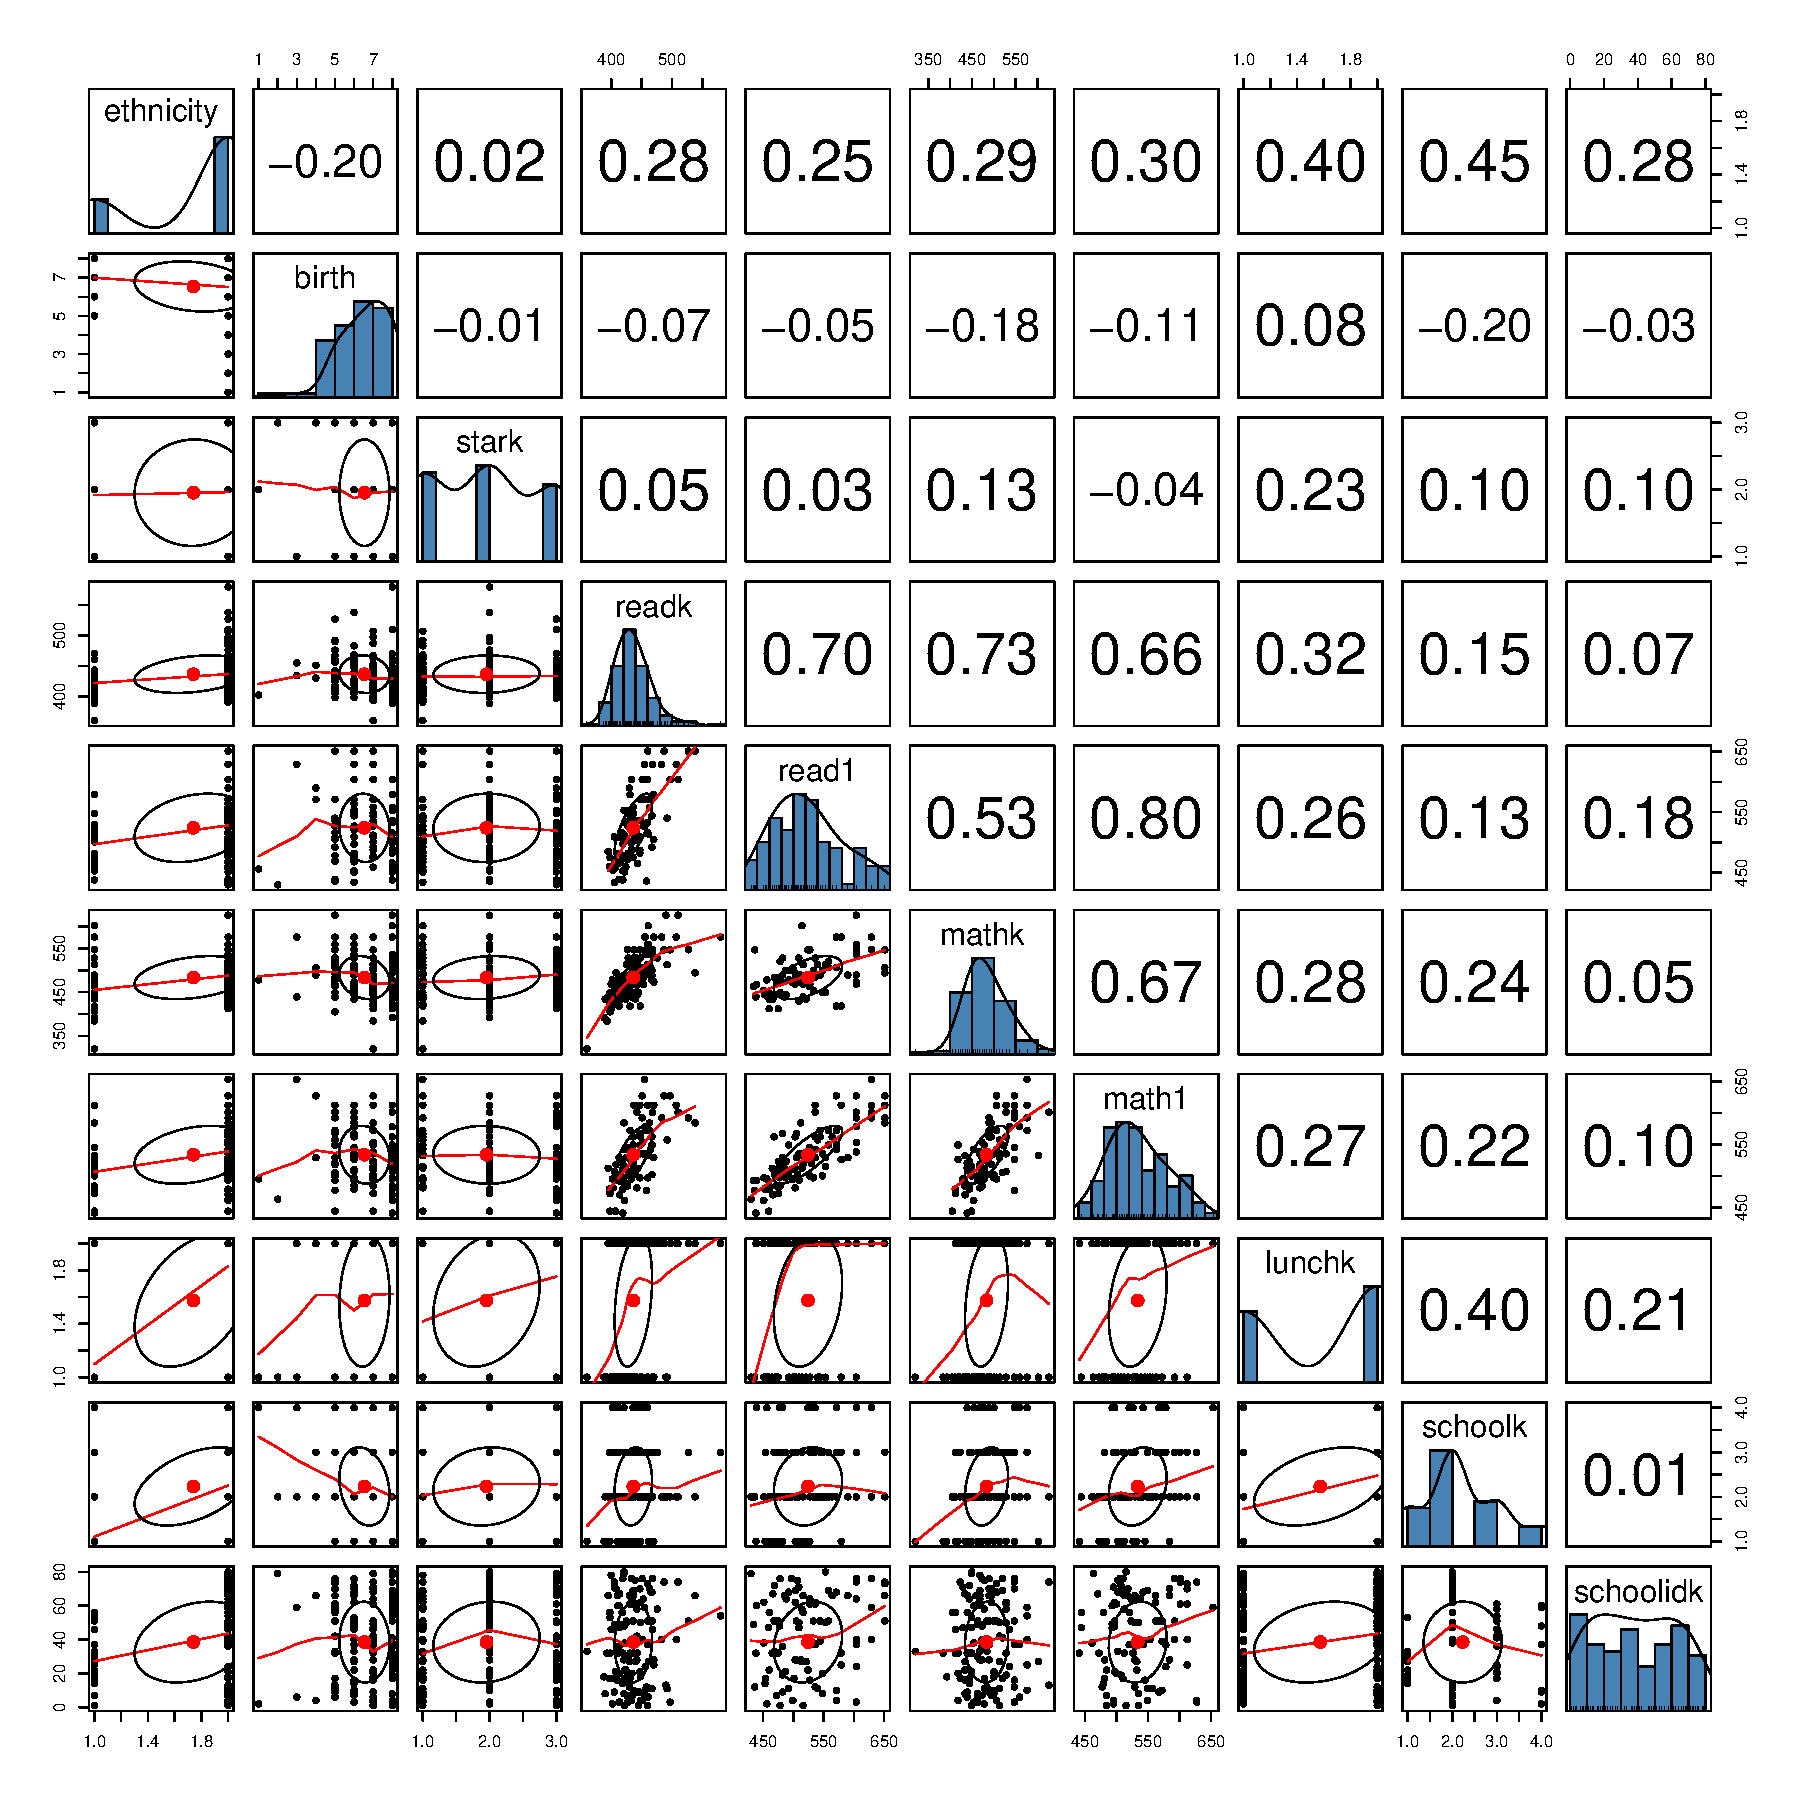
\includegraphics[width=\maxwidth]{figure/pairsplot} 


\clearpage
\section{Intent-to-treat Analyses}
\subsection{Pretest-posttest Regressions}

\begin{table}[h]
\begin{center}
\begin{tabular}{l c c }
\hline
                & Reading & Math \\
\hline
(Intercept)     & $108.84$    & $245.24^{***}$ \\
                & $(143.35)$  & $(53.38)$      \\
txtreatment     & $-0.71$     & $26.96^{**}$   \\
                & $(16.46)$   & $(9.35)$       \\
pretest         & $0.91^{**}$ & $0.53^{***}$   \\
                & $(0.32)$    & $(0.11)$       \\
gendermale      & $4.21$      & $16.90$        \\
                & $(17.58)$   & $(9.94)$       \\
ethnicitycauc   & $40.31$     & $34.05$        \\
                & $(29.33)$   & $(17.04)$      \\
degreekmaster   & $3.68$      & $16.59$        \\
                & $(20.79)$   & $(11.82)$      \\
degreekmaster+  & $-27.08$    & $-18.30$       \\
                & $(27.05)$   & $(15.69)$      \\
school1rural    & $-5.41$     & $-11.29$       \\
                & $(35.17)$   & $(20.29)$      \\
school1suburban & $-7.13$     & $-3.54$        \\
                & $(34.81)$   & $(20.31)$      \\
school1urban    & $-26.16$    & $-3.22$        \\
                & $(39.73)$   & $(23.01)$      \\
\hline
R$^2$           & 0.37        & 0.67           \\
Adj. R$^2$      & 0.16        & 0.56           \\
Num. obs.       & 36          & 37             \\
\hline
\multicolumn{3}{l}{\scriptsize{$^{***}p<0.001$, $^{**}p<0.01$, $^*p<0.05$}}
\end{tabular}
\caption{Unstandardized ITT Models}
\label{table:coefficients}
\end{center}
\end{table}





\begin{table}[h]
\begin{center}
\begin{tabular}{l c c }
\hline
                & Reading & Math \\
\hline
(Intercept)     & $-0.35$     & $-0.94^{**}$ \\
                & $(0.43)$    & $(0.29)$     \\
txtreatment     & $-0.01$     & $0.62^{**}$  \\
                & $(0.32)$    & $(0.21)$     \\
scale(pretest)  & $0.43^{**}$ & $0.54^{***}$ \\
                & $(0.15)$    & $(0.11)$     \\
gendermale      & $0.08$      & $0.39$       \\
                & $(0.34)$    & $(0.23)$     \\
ethnicitycauc   & $0.77$      & $0.78$       \\
                & $(0.56)$    & $(0.39)$     \\
degreekmaster   & $0.07$      & $0.38$       \\
                & $(0.40)$    & $(0.27)$     \\
degreekmaster+  & $-0.52$     & $-0.42$      \\
                & $(0.52)$    & $(0.36)$     \\
school1rural    & $-0.10$     & $-0.26$      \\
                & $(0.67)$    & $(0.46)$     \\
school1suburban & $-0.14$     & $-0.08$      \\
                & $(0.67)$    & $(0.47)$     \\
school1urban    & $-0.50$     & $-0.07$      \\
                & $(0.76)$    & $(0.53)$     \\
\hline
R$^2$           & 0.37        & 0.67         \\
Adj. R$^2$      & 0.16        & 0.56         \\
Num. obs.       & 36          & 37           \\
\hline
\multicolumn{3}{l}{\scriptsize{$^{***}p<0.001$, $^{**}p<0.01$, $^*p<0.05$}}
\end{tabular}
\caption{Standardized ITT Models}
\label{table:coefficients}
\end{center}
\end{table}



\clearpage
\clearpage
\begin{appendices}
\section{Data Preparation Code}
\label{rcode}
\subsection{starRmake.R}
\verbatiminput{../../../data/starRmake.R}
\subsection{prePost.R}
\verbatiminput{../../../analyses/prePost.R}
\subsection{stdPrePost.R}
\verbatiminput{../../../analyses/stdPrePost.R}
\clearpage
\section{R Session Information}
\begin{knitrout}
\definecolor{shadecolor}{rgb}{0.969, 0.969, 0.969}\color{fgcolor}\begin{kframe}
\begin{verbatim}
R version 3.0.2 (2013-09-25)
Platform: x86_64-pc-linux-gnu (64-bit)

locale:
 [1] LC_CTYPE=en_US.UTF-8       LC_NUMERIC=C              
 [3] LC_TIME=en_US.UTF-8        LC_COLLATE=en_US.UTF-8    
 [5] LC_MONETARY=en_US.UTF-8    LC_MESSAGES=en_US.UTF-8   
 [7] LC_PAPER=en_US.UTF-8       LC_NAME=C                 
 [9] LC_ADDRESS=C               LC_TELEPHONE=C            
[11] LC_MEASUREMENT=en_US.UTF-8 LC_IDENTIFICATION=C       

attached base packages:
[1] stats     graphics  grDevices utils     datasets  methods   base     

other attached packages:
[1] texreg_1.31       psych_1.4.2.3     reporttools_1.1.1 xtable_1.7-1     
[5] knitr_1.5        

loaded via a namespace (and not attached):
[1] evaluate_0.5.1 formatR_0.10   stringr_0.6.2  tools_3.0.2   
\end{verbatim}
\end{kframe}
\end{knitrout}

\end{appendices}
\end{document}
